\section{Auswertung}

Bevor wir mit der Aufzeichnung der eigentlichen Spektren begonnen haben, haben wir eine Dunkelstrommessung durchgeführt. Das Spektrum dieser ist in \abbref{fig:dunkelstrommessung} zu sehen.

\begin{figure}[H]
  \centering
  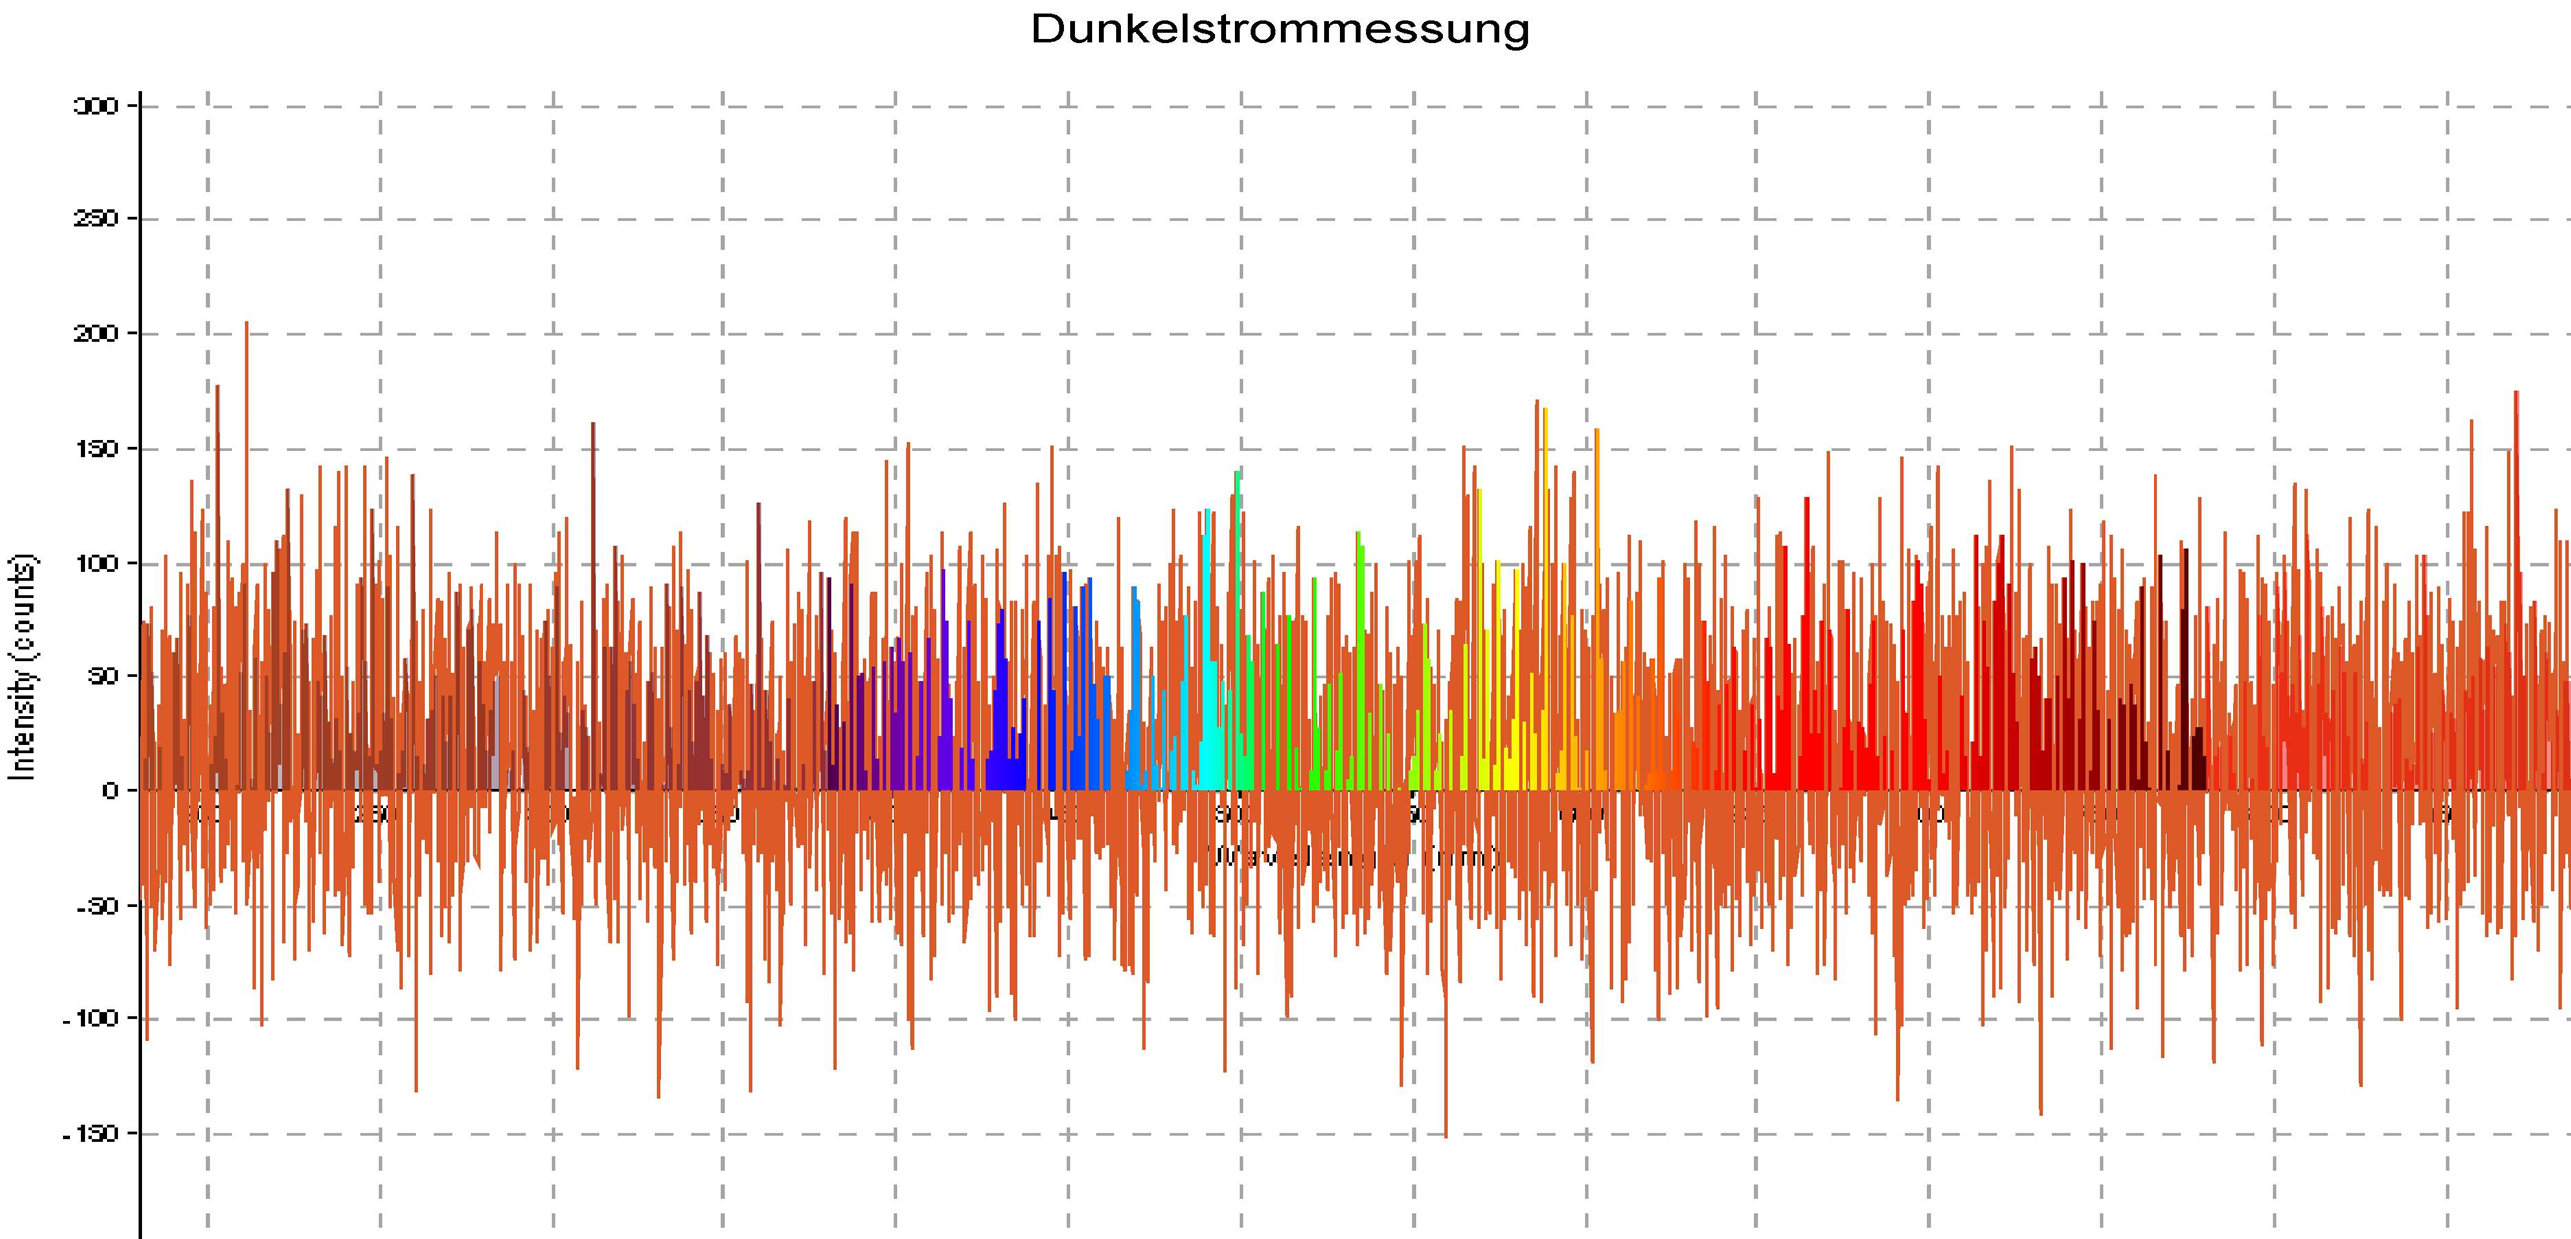
\includegraphics[width=.9\textwidth]{files/pngs/dunkelstrommessung.png}
  \caption{Spektrum Dunkelstrommessung}
  \label{fig:dunkelstrommessung}  
\end{figure}

Es handelt sich hierbei um ein Untergrundrauschen, welches wir mit der \texttt{OceanView} Software automatisch von allen weiteren aufgezeichneten Spektren abziehen.

\subsection{Untersuchung des Sonnenlichtspektrums}

Am Tag der Versuchsdurchführung war das Wetter leider stark bewölkt, weshalb wir mit dem Spektroskop nicht auf den blauen Himmel zielen konnten. Es ist also zu beachten, dass die folgenden Betrachtungen durch die Auswirkungen der Wolkendecke gestört sind. Die untenstehende \abbref{fig:himmel_m_o_g} zeigt aufgezeichnete Spektrum des Tageslichts durch das geöffnete Fenster (blau) und durch die Fensterscheibe (orange) im Vergleich. Es ist bereits hier zu sehen, dass die Intensität durch das Glas über das gesamte Spektrum hinweg abgeschwächt wird. Die stärkste Abschwächung verzeichnen wir bei niedrigen Wellenlängen, also im UV-Bereich. Dies ist auch am Verlauf der Absorption in \abbref{fig:absorption_glas} zu sehen. Die geringste Abschwächung tritt im Bereich der Wellenlänge zwischen $400$ bis $600\si{\nano\meter}$, also dem sichtbaren Bereich auf. In Richtung des Rot- bis Infrarotbereichs steigt die Absorption wieder etwas an.

\begin{figure}[H]
  \centering
  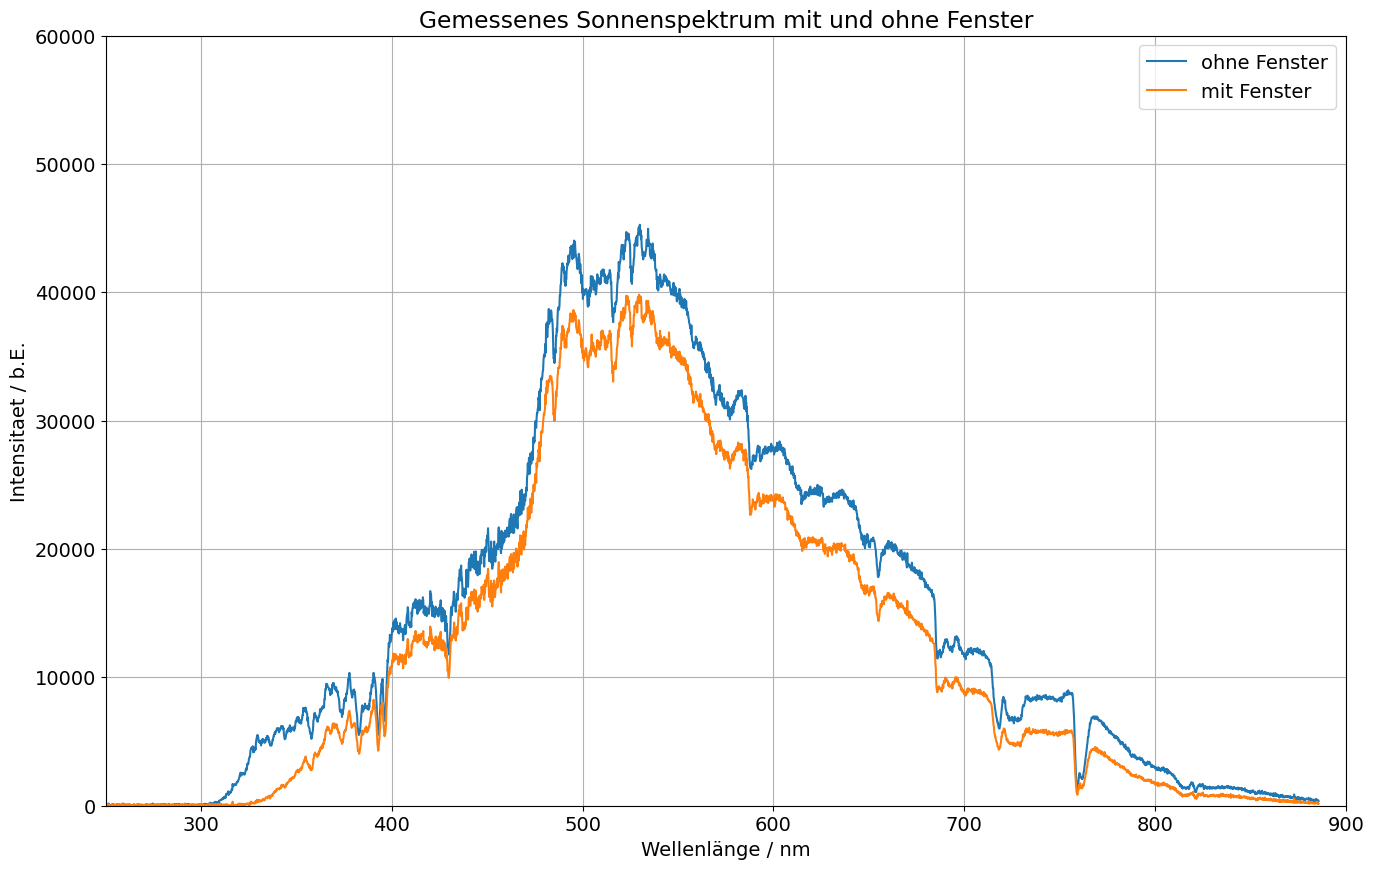
\includegraphics[width=0.8\textwidth]{files/plots/himmel_m_o_g.png}
  \caption{Sonnen}
  \label{fig:himmel_m_o_g}
\end{figure}

\begin{figure}[H]
  \centering
  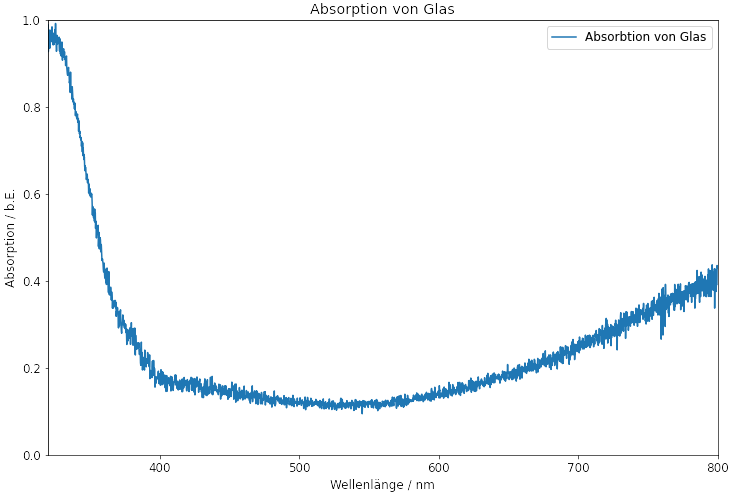
\includegraphics[width=0.8\textwidth]{files/plots/absorption_glas.png}
  \caption{Absorption}
  \label{fig:absorption_glas}
\end{figure}

Die vielen im Spektrum sichtbaren lokalen Minima sind gerade die Wellenlängen der Frauenhoferlinien, welche durch Absorption von Licht bestimmter Wellenlängen in der Sonnen- und Erdatmosphäre entstehen. \abbref{fig:spektrum_frauenhofer_balmer} zeigt erneut das Spektrum des Sonnenlichts, ohne Fensterscheibe. Markiert sind hier in Orange nun die Minima im Spektrum, welche jeweils am nächsten an der erwarteten Wellenlänge einer Frauenhoferlinie liegen. Zusätzlich sind in Grün die Literaturwerte der Wellenlänge der Balmer-Serie von Wasserstoff eingezeichnet.

\begin{figure}[H]
  \centering
  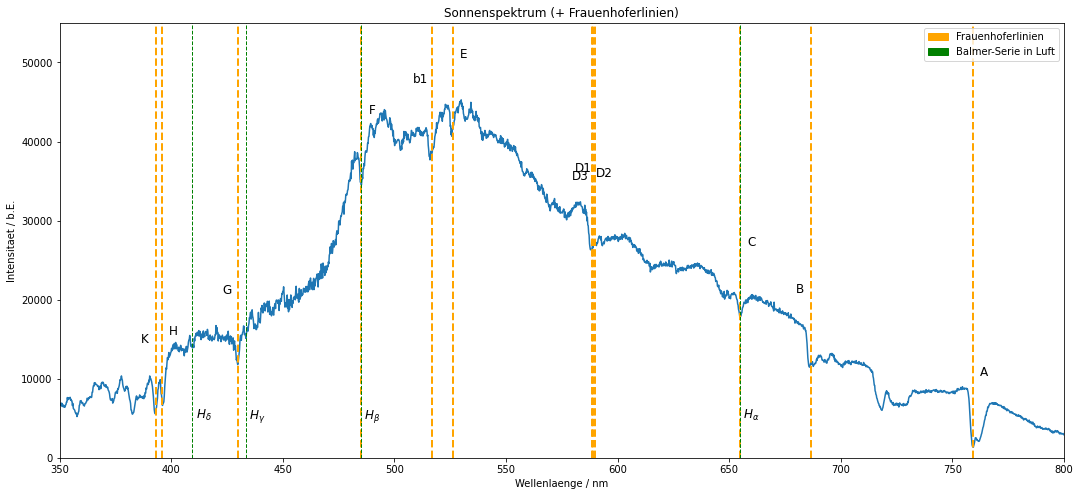
\includegraphics[width=\textwidth]{files/plots/spektrum_frauenhofer_balmer.png}
  \caption{Frauenhoferlinien und Balmerserie}
  \label{fig:spektrum_frauenhofer_balmer}
\end{figure}

\tabref{tab:frauenhofer_vergleich} zeigt eine Aufschlüsselung der erwarteten Wellenlänge der Frauenhoferlinien, die von uns aus dem Spektrum abgelesenen werte, sowie die Abweichung zwischen den Werten. Als Fehler für die abgelesenen Wellenlängen haben wir hier einen Wert von $\pm 1 \si{\nano\meter}$ verwendet. Es ist zu sehen, dass sich die Abweichung, bis auf wenige ausnahmen auf unter einem $\sigma$ beläuft.

\begin{table}[h]
  \centering
  \caption{Vergleich der erwarteten und gemessenen Wellenlängen der Frauenhoferlinien}
  \vspace*{0.5em}
  \begin{tabular}{c|c|c|c}
      \hline
      Linie & Literaturwert [nm] & Abgelesener Wert [nm] & Abweichung [$\sigma$] \\
      \hline
      K  & 393.4 & 393.0 & 0.4 \\
      H  & 396.8 & 396.1 & 0.7 \\
      G  & 430.8 & 429.8 & 1.0 \\
      F  & 486.1 & 485.2 & 0.91 \\
      b1 & 518.4 & 516.7 & 1.7 \\
      E  & 527.0 & 526.2 & 0.8 \\
      D3 & 587.6 & 588.4 & 0.8 \\
      D2 & 589.0 & 589.0 & 0.0 \\
      D1 & 589.6 & 589.7 & 0.11 \\
      C  & 656.3 & 655.0 & 1.3 \\
      B  & 686.7 & 686.7 & 0.0 \\
      A  & 759.4 & 759.4 & 0.0 \\
      \hline
  \end{tabular}
  \label{tab:frauenhofer_vergleich}
\end{table}

\newpage

\subsection{Vergleich der Spektren verschiedener Leuchtmitte}

Im Folgenden betrachten wir die Spektren verschiedener Lichtquellen. \abbref{fig:led_vergleich} zeigt hierzu zunächst die Spektren der drei untersuchen farbigen LEDs, sowie des Lasers.

\begin{figure}[H]
  \centering
  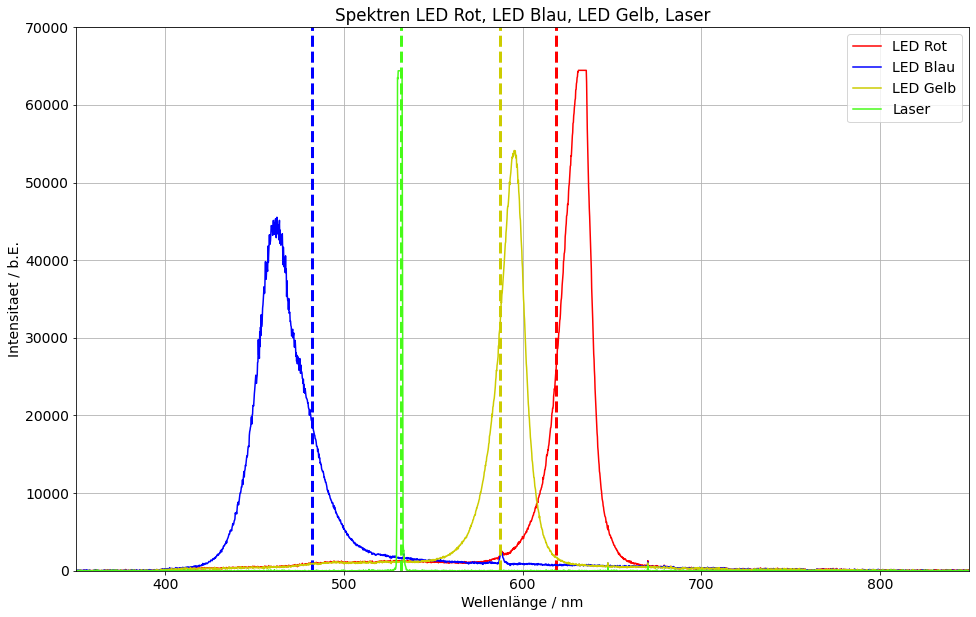
\includegraphics[width=.9\textwidth]{files/plots/led_vergleich.png}
  \caption{Aufgezeichnete Spektren der farbigen LEDs, sowie des Lasers.}
  \label{fig:led_vergleich}
\end{figure}

Die vertikalen Linien im Diagramm zeigen jeweils das nach Intensität gewichtete Mittel der Wellenlängen der Lichtquellen. Es ist zu erkennen, dass es sich hierbei in allen vier Fällen um diskrete Spektren handelt. Bei den LEDs streuen dabei die Wellenlängen etwas mehr und das Maximum der Verteilung ist etwas vom Mittel verschoben. Der Laser sendet konzentriertes Licht genau einer Wellenlänge aus, was sich ebenfalls an der direkten Überlagerung des \glqq{}Peaks\grqq{} mit dem Mittel zeigt.

Die Spektren der drei verschiedenen weißen LEDs sind gemeinsam mit dem der Energiesparlampe in \abbref{fig:led_und_energiespar} dargestellt. Alle vier Lichtquellen erzeugen, weitestgehend, weißes Licht. Am Spektrum der Energiesparlampe ist zu erkennen, dass diese das weiße Licht durch die Überlagerung mehrerer diskreter Wellenlängen erzeugt. Bei den weißen LEDs sehen wir jeweils einen relativ deutlichen, schmalen Peak bei den \glqq{}blauen\grqq{} Wellenlängen und einen sehr breiten Peak um den Bereich, in welchem Gelb zu verorten ist. Weiß wird hierbei also durch die Überlagerung von blauem und gelbem Licht erzeugt. Wir können außerdem beobachten, dass der Blau-Peak abnimmt, je \glqq{}wärmer\grqq{} das Weiß der LED wird. Durch geringere Blauanteile erhalten wir also wärmer erscheinendes Licht.

\begin{figure}[H]
  \centering
  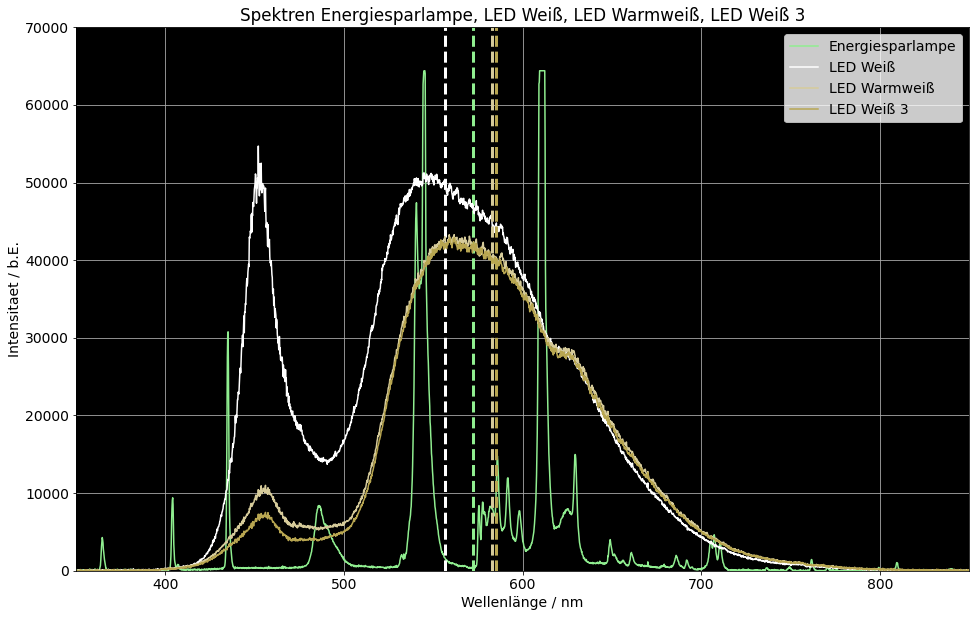
\includegraphics[width=.9\textwidth]{files/plots/led_und_energiespar.png}
  \caption{Aufgezeichnete Spektren der weißen LEDs, sowie der Energiesparlampe.}
  \label{fig:led_und_energiespar}
\end{figure}

Während die bisher betrachteten Lichtquellen Nichttemperaturstrahler sind, ist die Glühlampe ist ein Temperaturstrahler. Sie weist also ein kontinuierliches Spektrum auf, wie es auch in \abbref{fig:energiespar_und_glueh} zu sehen ist.

\begin{figure}[H]
  \centering
  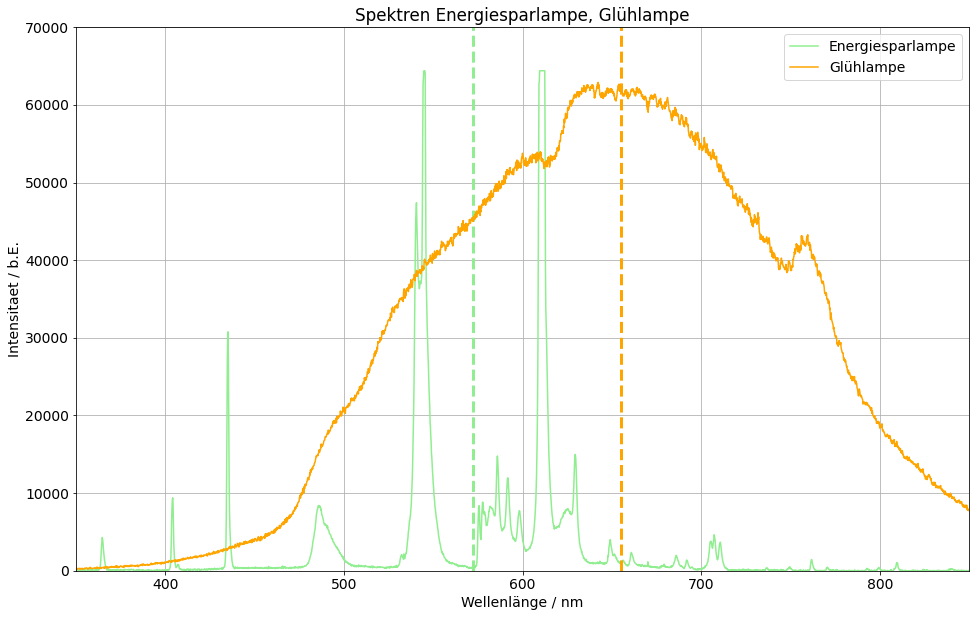
\includegraphics[width=.9\textwidth]{files/plots/energiespar_und_glueh.png}
  \caption{Aufgezeichnete Spektren der Glühlampe, sowie der Energiesparlampe.}
  \label{fig:energiespar_und_glueh}
\end{figure}

Am Spektrum der Glühlampe ist zu erkennen, dass sich ein nicht ungewisser Teil des Spektrums im oberen bis nicht sichtbaren Wellenlängenbereich befindet. Es geht hierbei also sehr viel Energie in Form von Wärme an die Umgebung verloren. Im Vergleich dazu ist die Energiesparlampe, deren Spektrum ebenfalls noch einmal in diesem Diagramm zu sehen ist, deutlich energieeffizienter. Die Glühlampe erzeugt eher ein warmes Licht, während die Lichttemperatur der Energiesparlampe eher in Richtung des kälteren Bereichs liegt.